% arXiv-ready LaTeX source for the LLM-Attacker paper.
% Compile: pdflatex main && pdflatex main   (self-contained, no .bib needed)
% Evidence scope and immutable release index: docs/paper-b-closure-2026-09-17.md.
\documentclass[11pt]{article}

\usepackage[utf8]{inputenc}
\usepackage[T1]{fontenc}
\usepackage{lmodern}
\usepackage[margin=1in]{geometry}
\usepackage{amsmath,amssymb}
\usepackage{tikz}
\usetikzlibrary{arrows.meta}
\usetikzlibrary{positioning}
\usepackage{booktabs}
\usepackage{array}
\usepackage{longtable}

\usepackage{graphicx}
\usepackage{xcolor}
\usepackage{microtype}
\setlength{\emergencystretch}{3em}

\usepackage{caption}
\PassOptionsToPackage{hyphens}{url}
\usepackage[colorlinks=true,linkcolor=blue,citecolor=blue,urlcolor=blue]{hyperref}
\usepackage{url}
\def\UrlBreaks{\do\/\do\-\do\.\do\_}

\newcommand{\pp}{pp}
\newcommand{\attack}[1]{\nolinkurl{#1}}
\newcommand{\eg}{e.g.\ }
\newcommand{\ie}{i.e.\ }

\title{The LLM-Attacker: A Unified Red-Team Framework for Privacy\\
Evaluation of Split and Distributed LLM Systems}

\author{Georgios Politis\\ {\small\texttt{geo.politis@gmail.com}} \and Setloop.io \and
  Evangelos Pappas\\ {\small\texttt{evanz.pappas@gmail.com}}}
\date{}

\begin{document}
\maketitle

\begin{abstract}
Privacy evaluation of split language models depends on the attacker's observations, model knowledge, computational budget and scoring rule. We present LLM-Attacker, a framework with 64 registered modules, a common command-line interface and artefact schema, versioned scoring, and tamper-evident execution records. Its modules cover reconstruction, property and membership inference, extraction, active attacks, side channels, and application and agentic security checks; registration does not imply matched reproduction or equal empirical validation. A frozen-protocol GPT-2 campaign comprises 3{,}680 logical cells over 40 attack arms. At depth six with a public head, joint activation--gradient observation improves token recovery over a matched activation-only baseline by 3.17 percentage points (95\% crossed-bootstrap interval [2.72, 3.64]), exceeding the prespecified two-point margin. Separately, a corrected white-box objective is evaluated at every internal GPT-2 boundary, depths one through eleven, with 198 stable-defence cells and 99 newly captured co-trained final-state cells. Descriptive domain, horizon and live-planner experiments illustrate the framework's scope and failure reporting. Historical claims from the August deployment and external defence campaigns are excluded because their source records remain unavailable. A separate matched BiSR validation establishes single-seam GPT-2 implementation conformance on a fixed fresh WikiText-103 holdout. Gate outputs are conditional operational diagnostics, not general privacy guarantees; untested settings, parser failures and excluded observations remain explicit.
\end{abstract}

\section{Introduction}
\label{sec:intro}

Split and distributed deployment of large language models (LLMs) includes
split fine-tuning, split inference and edge--cloud partition at a
\emph{seam} layer. Privacy motivates these designs: the untrusted host
receives boundary activations (`smashed data'), rather than raw text.
Whether those activations protect the text requires empirical evaluation
under a specified attacker. Comparisons across papers are difficult when
defences are tested against different attackers, budgets and scoring rules.

We present \textbf{LLM-Attacker}, a unified red-team framework for privacy
evaluation of split and distributed LLM training and inference. It makes
the attacker specification part of each claim. The registry covers
training-mode wires, inference-mode observations and the agentic deployment
stack, allowing evaluators to test defences across these surfaces. A defence verdict
is meaningful only when (i)~the attacker is stronger than or equal to the
published attack families it claims to resist, (ii)~the scoring rule is
frozen before the defence is designed, not tuned after, and (iii)~every
verdict is backed by an auditable artefact chain that a second party can
re-derive cell by cell. Recent work demonstrates dual-sided leakage of input prompts and generated responses \cite{gu2026pidi}. Comparing defences against such attacks requires explicit, consistent attacker capabilities and observation grants.

\newpage
\paragraph{Contributions.}
\begin{enumerate}
\item \textbf{A unified, extensible attacker framework.}
  64 registered attack modules under one CLI, one artefact schema
  (\texttt{schema}/\texttt{config}/\texttt{threat\_model}/
  \texttt{provenance}/\texttt{results}/\texttt{summary}), crash-safe
  per-cell JSONL journals, a tamper-evident evidence chain, a plugin API
  for third-party attacks, and an observation-surface registry so adapters can support new
  capture formats (vRAM, timing, wire shape) without forking the loader
  (\S\ref{sec:framework}).
\item \textbf{A frozen scoring gate.}
  A versioned, retargetable gate: excess of the
  Bonferroni-adjusted Wilson upper-95 of the best attack arm over a
  label-free majority control must stay $\le +1.0$~\pp, with an explicit
  statistical-floor analysis (computed from the control rate and sample size), a three-seed requirement, and per-cell control-rate and statistical-floor reporting. Any change to the constants requires a new named gate version;
  archived verdicts retain their recorded versions, while the implementation's current default is \texttt{frozen-gate.v2} (\S\ref{sec:gate}).
\item \textbf{A traceable real-model evaluation.}
The canonical v3 campaign tests a prespecified joint-observation contrast, while separate GPT-2 domain and horizon experiments report their own controls, budgets and statistical limitations (\S\ref{sec:deployment}). Paper~A shares the v3 evidence; it is not an independent replication.
\item \textbf{A corrected all-boundary white-box evaluation.}
The attack objective includes the client head between optimised embeddings and the defence encoder. A matched 36-cell rerun precedes a descriptive sweep of all eleven internal GPT-2 boundaries. Newly captured co-trained observations use matched final checkpoints and a separately labelled access grant (\S\ref{sec:whitebox}).
\end{enumerate}

\paragraph{Scope and ethics.}
The framework is a red-team \emph{evaluation} tool: every attack runs a
torch-free toy tier for machinery checks on any laptop, and real runs
operate on captures produced by systems the evaluator controls (our own
split harness, our own fleet, or a man-in-the-middle relay on our own
link). Its purpose is to make privacy claims testable under explicit attack conditions. Application-layer and agentic risks are evaluated under
separate named profiles (\S\ref{sec:coverage}), to keep split-seam and application-layer claims distinct; the agentic profile is
out of scope by default unless tool, memory, and action surfaces exist.

\section{Threat Model}
\label{sec:threat}

Three independent axes organise the attacker space; every module declares
its coordinates and restates them in its artefact's \texttt{threat\_model}
field, so a verdict always carries the assumptions under which it was
obtained. These coordinates are machine-checkable: each
module carries validated registry metadata (actor intent, persistence,
observation surfaces, security properties, lifecycle stage, framework
mappings; enforced over the whole registry in CI), and the artefact field
itself is a versioned, validated document
(\texttt{llm\_attacker.threat\_model.v2}) with legacy strings normalised,
so threat assumptions are comparable across runs and attacks.

\paragraph{Axis 1: honest-but-curious vs.\ active/malicious.}
The default attacker is a passive cloud participant that performs the specified
computation and observes wire tensors. The \emph{active-cloud} axis drops that assumption:
the cloud injects crafted perturbations into returned tensors or, during
training, modifies optimiser updates and body computations to increase
leakage from the local node. This adapts the federated-learning
malicious-server threat to split learning.

\paragraph{Axis 2: labelled vs.\ label-free.}
\emph{Labelled} attackers obtain (activation, known-token) pairs -- via an
oracle, chosen plaintext, or self-labelled replay -- and have strictly more information than the default attacker. Their
recovery curves describe that additional grant, rather than the default
threat model. \emph{Label-free} attackers use only
public text and public base weights.

\paragraph{Axis 3: per-epoch vs.\ cross-epoch.}
Per-epoch rotation of the seam secret resets the honest accumulation
window. Cross-epoch attackers retain information across rotations: they exploit a shared stable
subspace (\attack{subspace-joint}), accumulate leaked key material across
rotations (\attack{leak-accumulation}), or arrive holding stale keys
(\attack{stale-key}). The methodology requires that cross-epoch pooling
controls sit in the label-free band -- otherwise the per-epoch budget
accounting is invalid.

\paragraph{Vantage points.}
The same attack modules run in three deployment shapes without code
changes: (i)~\emph{localhost}, installed next to the defence;
(ii)~\emph{remote}, probing a fleet (two GPU nodes, three CPU nodes in our
deployment) and pulling capture directories over SSH with per-node
degradation instead of crashes; and (iii)~\emph{man-in-the-middle}, a TCP
relay that tees both directions of the local$\leftrightarrow$cloud link
into a wire-shape journal, never throttling over-cap traffic so capture
cannot perturb the observed system.

\section{The Unified Framework}
\label{sec:framework}

\subsection{One registry, one schema, one journal}

Every attack is an independent module behind one CLI
(\texttt{python -m attacker --mode M --attack NAME}, with \texttt{M} one of
\texttt{training}/\texttt{inference}),
registered under a validated contract (\texttt{EXPERIMENT\_ID},
\texttt{MODES}, \texttt{REQUIRES\_LABELS}, \texttt{DESCRIPTION},
\texttt{build\_parser}, \texttt{run}). Third-party attacks join through the
\texttt{llm\_attacker.attacks} entry-point group or programmatic
registration; a name collision raises a descriptive error instead of overriding an
existing module. The mode flag selects the wire-capture sidecar schema
(training-mode records carry micro-batch/step/epoch metadata;
inference-mode records carry request-sequence/position metadata), and the
two historical schemas are built-in providers of an observation-surface
registry: a provider declares its metadata keys and yields
(tensor, metadata) rows, so an adapter can add surfaces such as GPU-memory residue, kernel
timing or traffic shape without forking the capture loader.

Run outputs comprise two standard records and an optional evidence chain:
\begin{enumerate}
\item \textbf{One JSON artefact} with fixed top-level fields
  (\texttt{schema}, \texttt{config}, \texttt{threat\_model},
  \texttt{provenance}, \texttt{results}, \texttt{summary});
\item \textbf{A crash-safe JSONL journal} appended after every experiment
  cell, so partial results survive host failures and optimisation-loop
  attacks resume after crashes;
\item \textbf{Optionally, a tamper-evident evidence chain}
  (\texttt{--evidence}): a hash-chained event log (each event's
  SHA-256 covers the previous hash) plus a run manifest capturing argv,
  UTC timestamps, host/platform/python, installed package versions, git
  commit and dirty flag, and the artefact hash. Auditors re-derive the
  chain with \texttt{verify\_evidence(path)}; any modified, deleted, or
  reordered event fails verification with the exact location named.
\end{enumerate}

Numerical failures in the solve routines return structured
\texttt{error:\ ...} records and are journalled per cell, preserving the
failure for inspection. The shared solve core enforces
contiguous-float64 discipline for the polar least-squares key solves that
most capture-side attacks reduce to.

\subsection{Torch-free baseline and toy tiers}

The framework's import surface is torch-guarded: \texttt{--help},
\texttt{--list-attacks}, and \texttt{--self-test} (per-module pure-Python
frozen fixtures) run with no deep-learning stack installed, and CI
runs the self-test as a subprocess to enforce this constraint. Every
attack additionally implements a \texttt{--toy --quick} tier on synthetic
tensors, which exercises capture loading, solving,
gate integration and artefact writing on any laptop in minutes. Toy results
are machinery checks, \emph{never} security claims; the distinction is
enforced by convention and restated in every artefact's provenance.

\subsection{The split harness}

To support joint development of attackers and defences, the framework includes a
split-LLM harness (\texttt{splitbench}): GPT-2-class models partitioned as
head\,|\,body\,(|\,tail), optional LoRA adapters, and a reference defence
pack (Gaussian seam noise at public $\sigma$, top-$k$ sparsification,
mid-lite bottlenecking, sanitisation, activation trimming) emitting the
native wire-capture schema. A capture run can supply every attacker, allowing
$N$ attacks $\times M$ hosts to run in parallel. Capture generation requires
defence-side forward passes; subsequent attacks solve against cached rows.

\subsection{Explicit coverage reporting}
\label{sec:coverage}

Reporting only completed attacks can obscure gaps in an assessment. The framework therefore separates \emph{measurement} from
\emph{coverage}. \texttt{--coverage} aggregates run artefacts into a
manifest in which every threat in the framework's threat universe -- the
S1--S14 surfaces of Table~\ref{tab:surfaces} and the OWASP LLM 2026
Top~10 \cite{owasp2026asi} -- is reported as exactly one of \textbf{COVERED} (every mapped
attack produced a valid result), \textbf{PARTIAL} (some mapped attacks
ran; the untested ones are named), \textbf{UNMEASURED} (applicable but
untested), or \textbf{OUT\_OF\_SCOPE} (explicitly inapplicable, with a
documented reason). UNMEASURED and OUT\_OF\_SCOPE are never conflated,
and an error-only cell counts as no result: a failed attack does not
count towards coverage.

\texttt{--profiles} groups the threats into versioned benchmark profiles:
\texttt{benchmark.split-privacy.v2} (the S1--S9 privacy families plus
tenant isolation, artefact/telemetry leakage, and the router side channel,
with \attack{privacy-composition} as the final composite cell),
\nolinkurl{benchmark.split-integrity-availability.v1} (protocol integrity,
malicious client and server, poisoning/backdoor, resource exhaustion,
key/session abuse, supply chain), \texttt{benchmark.genai-app.v1} (the
OWASP LLM01--LLM10 manifest), and \texttt{benchmark.agentic.v12} (OWASP
ASI01--ASI10, requiring the ten agentic modules and cross-agent-deputy -- \attack{agent-goal-hijack}, \attack{tool-misuse},
\attack{identity-privilege-abuse}, \attack{agentic-supply-chain},
\attack{unexpected-code-execution}, \attack{memory-context-poisoning},
\attack{insecure-agent-communication}, \attack{cascading-failure},
\attack{human-agent-trust}, \attack{rogue-agent}, and \attack{cross-agent-deputy} -- sandboxed agents scored by policy-layer effect, each defence proven
load-bearing by single-flag ablation) -- the last OUT\_OF\_SCOPE by
default because the framework
evaluates split/distributed LLMs without tool, memory, or inter-agent
surfaces, and becomes applicable only for agentic targets. The standard
battery (\texttt{benchmark.v1}) remains the frozen environment grader for
S1/S2/S5/S9; coverage beyond those axes is reported through the manifest,
never implied by the battery.

\section{The Frozen Gate}
\label{sec:gate}

The methodological core is a scoring rule that is fixed \emph{before}
defences are designed and never moves while they evolve.

\noindent\textbf{Definition (numerical rule, current \texttt{frozen-gate.v2}).}
For an attack arm with recovery $\hat{p}$ on $n$ evaluation rows and a
label-free majority control $p_0$ (the mode of training labels applied to
evaluation rows), the \emph{excess} is
\[
\mathrm{excess} \;=\;
100 \times \bigl( U_{95}(\hat{p}, n) - p_0 \bigr)
\quad\text{percentage points},
\]
where $U_{95}$ is the one-sided Wilson upper confidence bound with
Bonferroni-corrected $z = 2.5392$ ($\alpha = 0.05$ over 9 trials: 3 model
classes $\times$ 3 restarts). The reported cell score is the
\emph{worst} (highest) arm's excess. A defence \textbf{PASS}es iff
$\mathrm{excess} \le +1.0$~\pp{} and the verdict is backed by $\ge 3$
seeds.

Three properties govern interpretation:

\paragraph{The statistical floor is reported.}
When recovery equals the label-free control rate, the upper-bound excess remains positive at finite sample sizes. This statistical floor is computed per cell from the control rate, row count and gate constants; it is not a universal minimum, because recovery below control can yield smaller or negative excess. The artefact records the floor and an \texttt{at\_floor} flag. The control rate must be read alongside the verdict. The generic gate does not currently enforce a corpus-specific minimum control rate: the previously promised automatic suppressed-control flag is not implemented.

\paragraph{The control is label-free.}
Majority-token guessing supplies an explicit comparator without the victim model. Calibration must be declared. In the historical long-horizon battery the synthetic-calibration majority token never occurs in the evaluation text, yielding a zero control rate; this is a limitation of that battery, not evidence that the corpus has no predictable tokens. The newer domain experiments report per-corpus controls.

\paragraph{Changes require a new version.}
The constants live in \texttt{GateConfig}; changes to significance level, trial family, threshold or seed requirement require a named version. The current \texttt{frozen-gate.v2} uses the stated numerical rule and refuses PASS below three declared seeds. Recorded historical verdicts retain their executed versions. We do not assert that every historical report used identical constants or that its verdict survives re-issuance; the retained long-horizon summary includes both historical and current-constant recalculations. A gate version alone does not make different corpora, budgets or observation grants comparable.

\paragraph{CI enforcement.}
\texttt{--scorecard} aggregates artefacts into one report (per-cell
verdict, worst cell, error cells surfaced) and exits 1 when any cell
FAILs, enforcing the gate in the build.

\paragraph{What a gate verdict does and does not say.}
This paper reports three different forms of evaluation, and they support
different conclusions. The historical token-level gate above is an
\emph{operational diagnostic}: it is conditional on its sampling scheme,
its label-free majority control, and its correction family, and the token
observations within a cell are clustered rather than independent. A PASS
means that no tested arm's upper confidence bound on excess recovery rose
above the threshold under those assumptions -- it is not a general
privacy certificate. Two further restrictions apply. The $+1.0$~\pp{}
threshold governs token-recovery excess only; membership AUC,
distillation $R^2$, timing channels, and agentic tool-action rates carry
endpoint-specific treatments and are never passed through this
threshold.

A PASS also requires a positive control:
the same attacker must exceed control on an undefended reference target
(the framework's positive-control battery,
\nolinkurl{results/attacker-positive-controls-v1/}), to check that an ineffective attack implementation does not account for
the PASS. The scorecard
enforces this requirement: under the default \texttt{scorecard-policy.v3} (the
numeric gate remains \texttt{frozen-gate.v2}), a PASS stands only
alongside a linked positive-control artefact whose re-validated excess
exceeds the threshold on an undefended reference target; a PASS without
one is downgraded to INSUFFICIENT\_EVIDENCE (exit 2, fail-closed), and
\texttt{--scorecard-policy scorecard-policy.v2} reproduces the
pre-requirement behaviour for legacy bundles.

A verdict is specific to its corpus and configuration: the domain experiment in \S\ref{sec:deployment} reports different control rates and recovery magnitudes, so a PASS does not transfer to a different corpus or domain
without re-evaluation under a pinned, hashed corpus. Conversely, a FAIL can reflect an imprecise upper
bound as much as demonstrated excess leakage.

The v3 campaign of
\S\ref{sec:v3} is a different instrument: prespecified paired
contrasts with a crossed bootstrap over documents and victim runs,
supporting bounded inference about attack \emph{differences}. The defence,
span, perturbation, and utility-cost summaries accompanying it are
\emph{descriptive} comparisons under the frozen protocol and carry no
inferential claim. We label each form of evaluation explicitly; the successful
v3 analysis neither repairs nor replaces the historical gate's
assumptions.

\section{Anatomy and Categorisation of the Attack Space}
\label{sec:taxonomy}

\subsection{Anatomy: where the attacks hit}

Figure~\ref{fig:anatomy} shows the system under attack: a decoder-only LLM
partitioned at a \emph{seam} between the victim (data owner) and the cloud
(compute). Nine observation surfaces (S1--S9) form the seam-centric surface model -- the in-scope enumeration of what an adversary can observe at the split
boundary; control-plane metadata, persistent stores, and MoE router state
extend it. Table~\ref{tab:surfaces} maps each surface to the attack families
that exploit it. Two structural facts drive the design of the battery.
First, the seam is bidirectional: the forward activation $h^{*}$ (S1) and
the backward seam gradient $\partial\mathcal{L}/\partial h^{*}$ (S2) are
different surfaces -- a defence that transforms only one still faces the
full family on the other (the \texttt{joint} arm of
\attack{seam-inversion} can exploit both at once in a causal beam). Autoregressive generation also permits dual-sided leakage of inputs and generated responses \cite{gu2026pidi}. Second, depth is an experimental condition: the corrected GPT-2 sweep
varies across internal boundaries (Section~\ref{sec:whitebox}). A split
point alone is not a privacy certificate. Methods based on continuous theoretical metrics, such as Fisher information, also seek to measure and control leakage \cite{maeng2022refil}. Here we evaluate realised leakage using discrete structural inference attacks.

\begin{figure}[tp]
\centering
\resizebox{0.96\textwidth}{!}{%
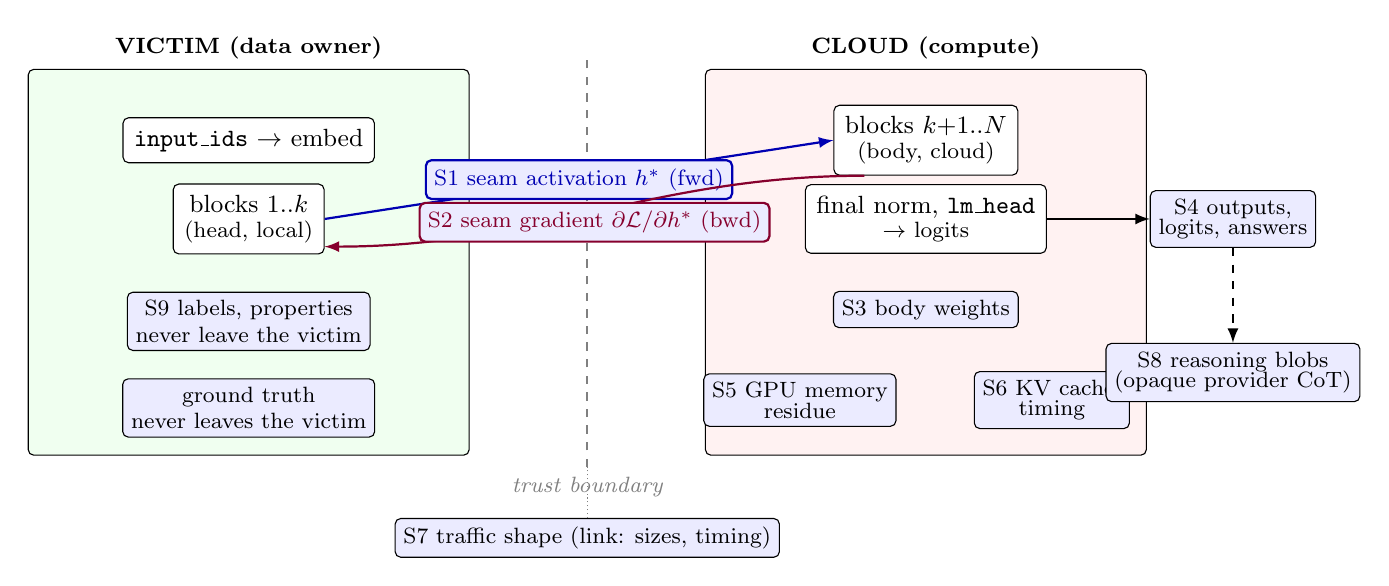
\begin{tikzpicture}[
  font=\small,
  box/.style={draw, rounded corners=2pt, align=center, inner sep=4pt},
  surf/.style={draw, fill=blue!8, rounded corners=2pt, align=center,
               inner sep=3pt, font=\footnotesize},
  wire/.style={-{latex}, thick},
  every node/.style={align=center}
]
% victim side
\node[box, fill=green!6, minimum width=5.6cm, minimum height=4.9cm,
      label={[font=\footnotesize\bfseries]above:VICTIM (data owner)}]
      (victim) at (0,0) {};
\node[box, fill=white] (wte) at (0,1.55)
      {\texttt{input\_ids} $\to$ embed};
\node[box, fill=white] (head) at (0,0.55)
      {blocks $1..k$\\[-2pt]\footnotesize (head, local)};
\node[surf] (s9) at (0,-0.75)
      {S9 labels, properties\\\footnotesize never leave the victim};
\node[surf] (gt) at (0,-1.85)
      {ground truth\\\footnotesize never leaves the victim};
% cloud side
\node[box, fill=red!5, minimum width=5.6cm, minimum height=4.9cm,
      label={[font=\footnotesize\bfseries]above:CLOUD (compute)}]
      (cloud) at (8.6,0) {};
\node[box, fill=white] (body) at (8.6,1.55)
      {blocks $k{+}1..N$\\[-2pt]\footnotesize (body, cloud)};
\node[box, fill=white] (tail) at (8.6,0.55)
      {final norm, \texttt{lm\_head}\\[-2pt]\footnotesize $\to$ logits};
\node[surf] (s3) at (8.6,-0.6) {S3 body weights};
\node[surf] (s5) at (7.0,-1.75) {S5 GPU memory\\[-2pt]\footnotesize residue};
\node[surf] (s6) at (10.2,-1.75) {S6 KV cache,\\[-2pt]\footnotesize timing};
% the seam
\draw[dashed, thick, gray] (4.3,-2.6) -- (4.3,2.6)
      node[below, font=\footnotesize\itshape, gray] at (4.3,-2.6) {trust boundary};
\draw[wire, blue!70!black] (head.east) -- node[surf, midway] (s1)
      {S1 seam activation $h^{*}$ (fwd)} (body.west);
\draw[wire, purple!70!black] (body.210) to[out=180,in=0]
      node[surf, midway, yshift=-4pt] (s2)
      {S2 seam gradient $\partial\mathcal{L}/\partial h^{*}$ (bwd)}
      (head.340);
% outputs
\node[surf] (s4) at (12.5,0.55) {S4 outputs,\\[-2pt]\footnotesize logits, answers};
\draw[wire] (tail.east) -- (s4.west);
% reasoning API inset
\node[surf] (s8) at (12.5,-1.4) {S8 reasoning blobs\\[-2pt]
      \footnotesize (opaque provider CoT)};
\draw[wire, dashed] (s4.south) -- (s8.north);
% traffic shape on the link
\node[surf] (s7) at (4.3,-3.5) {S7 traffic shape (link: sizes, timing)};
\draw[densely dotted, gray] (s7.north) -- (4.3,-2.6);
\end{tikzpicture}}
\caption{Anatomy of a split LLM under attack. The victim holds the
embedding and head blocks plus all ground truth; the cloud holds the body
and output stack. Surfaces S1--S9 are the seam-centric observation model (the control plane,
stores, and router surfaces extend it);
Table~\ref{tab:surfaces} assigns the attack families. The 3-slice variant
(head\,|\,body\,|\,tail) adds a second forward seam; MoE bodies leave the
seam tensor unchanged but add router decisions as a candidate leak
channel.}
\label{fig:anatomy}
\end{figure}

\begin{table}[!htp]
\centering\small
\caption{The attack-surface map: what crosses each surface of
Figure~\ref{fig:anatomy} and which modules attack it.}
\label{tab:surfaces}
\footnotesize
\begin{tabular}{@{}clp{4.2cm}p{6.1cm}@{}}
\toprule
\# & Surface & What crosses it & Attacks on it \\
\midrule
S1 & seam activations (fwd) & $h^{*}$ per microbatch / prefill &
\attack{seam-inversion}, \attack{vec2text-inversion}, rotation-era family,
latent battery, \attack{wire-eval} \\
S2 & seam gradients (bwd) & $\partial\mathcal{L}/\partial h^{*}$ &
\attack{gradient-inversion} (DLG++/iDLG/TAG), \attack{batch-label-recon},
\attack{label-scoring}, \texttt{joint} arm \\
S3 & body weights & never (held by cloud) &
\attack{body-extraction} (functional distillation) \\
S4 & outputs / logits / answers & API responses &
\attack{output-inversion}, \attack{trace-inversion} \\
S5 & GPU memory residue & freed buffers, local memory &
\attack{gpu-memory} (residue, scrub-check) \\
S6 & cache / timing & KV/prefix cache, contention, acceptance patterns &
\attack{kv-timing} (\texttt{spec-decode} arm), \attack{gpu-memory}
(\texttt{um-timing} arm) \\
S7 & traffic shape & packet sizes/timing on the link &
\attack{wire-shape} (via \attack{mitm-proxy} capture) \\
S8 & API reasoning blobs & encrypted CoT envelopes &
\attack{reasoning-replay} \\
S9 & labels / properties & never directly &
\attack{lira-membership}, \attack{membership}, \attack{label-scoring} \\
\midrule
\multicolumn{4}{@{}l}{\emph{Extended surfaces (threat-model review,
\S\ref{sec:coverage}):}}\\
S10 & protocol / control plane & negotiation, session binding, epochs, keys &
\attack{protocol-integrity}, \attack{key-session-abuse},
\attack{seed-disclosure} \\
S11 & persistent stores / telemetry & captures, logs, checkpoints, crash
dumps, backups & \attack{artifact-telemetry-leak}, \attack{remote-fetch} \\
S12 & MoE router metadata & expert IDs, queue depth, capacity overflows &
\attack{router-side-channel} \\
S13 & AI artefacts / supply chain & models, tokenisers, adapters, datasets,
plugins & \attack{supply-chain}, \attack{poisoning-backdoor} \\
S14 & application context & system prompts, RAG documents, tool schemas,
memory & \attack{prompt-injection}, \attack{hidden-context-exposure},
\attack{rag-vector-abuse} \\
\bottomrule
\end{tabular}
\end{table}

\subsection{Categorisation: surfaces, vantages, families}

The registry locates each module within three complementary categorisations:

\paragraph{By surface (Table~\ref{tab:surfaces}).} Which observable the
attack consumes. This is the defender's checklist: protecting S1 while
leaving S2, S6, or S7 open leaves those attack surfaces exposed.

\paragraph{By vantage point.} What position the attacker must hold:
\textbf{(A)~co-tenant} on the victim host (\attack{gpu-memory});
\textbf{(B)~inline} on the wire path (\attack{mitm-proxy},
\attack{wire-shape}); \textbf{(C)~server-side}, the attacker \emph{is} the
cloud (\attack{active-cloud}, \attack{malicious-server});
\textbf{(D)~files-only}, offline analysis of captured tensors and stores -- the honest-but-curious cloud already owns these, so this is the default
vantage of the bulk of the registry, and the explicit one of
\attack{artifact-telemetry-leak}; and \textbf{(E)~external API
client} (\attack{reasoning-replay}, \attack{trace-inversion},
\attack{kv-timing} endpoint mode, \attack{body-extraction} query access).
The deployment determines which vantage points are relevant:
co-tenant GPUs face S5/S6; multi-tenant serving faces S6; any reasoning
API faces S8.

\paragraph{By family (Table~\ref{tab:taxonomy}).} The mechanism shared by
a group of modules: rotation/key-era cryptanalysis, inversion, membership
and property inference, the latent-defence battery, the systems/hardware
seam, reasoning theft, active-cloud, and meta/evaluation drivers.

The framework runs separate attackers on a shared capture harness, in
parallel across hosts, and reserves a composite cell for the final
worst-case stress test. Separate attackers support claims about individual
mechanisms; composition (\eg{} \attack{alignment-search} harvesting pairs
\emph{for} \attack{accumulation}, or \attack{max-effort} wrapping the
strongest cell with swept budgets and full distributions instead of means)
supplies the final composite assessment of a defence.

{\small
\begin{longtable}{@{}p{2.9cm}p{4.1cm}p{1.1cm}p{5.6cm}@{}}
\caption{Attack families in the LLM-Attacker (64 registered modules).
Modes: T = training, I = inference. Entries describe implemented capabilities or explicitly scoped evaluations; they are not a uniform validation of attack strength. Historical August and external defence-campaign numerical highlights have been removed because their required source records remain unavailable. Application and agentic simulator checks are separate from live-model evidence (\S\ref{sec:agenticlive}).}
\label{tab:taxonomy}\\
\toprule
Family & Modules & Modes & Capability / evidence scope \\
\midrule
\endfirsthead
\caption[]{Attack families in the LLM-Attacker (continued).}\\
\toprule
Family & Modules & Modes & Capability / evidence scope \\
\midrule
\endhead
\midrule
\multicolumn{4}{r@{}}{\footnotesize continued overleaf}\\
\endfoot
\bottomrule
\endlastfoot
Trained inversion &
\attack{latent-probe} (9 arms), \attack{latent-sensitivity},
\attack{vec2text-inversion}, \attack{seam-inversion} &
T, I &
Trained and optimisation-based reconstruction; v3 and corrected white-box results have separate observation grants and budgets \\
\addlinespace[2pt]
Matching attacks &
\attack{latent-matching} (VMA-centroid, position-free signature) &
T &
Centroid and position-free signature matching; synthetic token and order endpoints are retained separately \\
\addlinespace[2pt]
Key / budget solves &
\attack{accumulation}, \attack{stale-key}, \attack{sharded},
\attack{leak-accumulation}, \attack{subspace-joint}, \attack{wire-eval},
\attack{seed-disclosure} &
T, I &
Known-pair budgets, cross-epoch pooling and key-lifetime controls; no external defence verdict asserted \\
\addlinespace[2pt]
Known-plaintext &
\attack{known-prefix}, \attack{alignment-search} (DTW/edit realignment) &
T, I &
Known-prefix solves and edit-distance/DTW realignment under declared label and alignment grants \\
\addlinespace[2pt]
Gradient / output &
\attack{gradient-inversion} (DLG++, iDLG, prior, TAG arms),
\attack{output-inversion}, \attack{label-scoring},
\attack{batch-label-recon} &
T, I &
Gradient/output reconstruction and norm-based property scoring; historical Mistral headline measurements excluded \\
\addlinespace[2pt]
Membership &
\attack{membership}, \attack{lira-membership} (LiRA/RMIA scoring) &
T &
LiRA/RMIA-style score aggregation with null-world controls; no matched published-method superiority claimed \\
\addlinespace[2pt]
Structure / blind &
\attack{ica-bss} (pure-torch FastICA) &
T, I &
Higher-order blind-source separation beyond covariance-based attacks \\
\addlinespace[2pt]
Active / malicious &
\attack{active-cloud}, \attack{malicious-server} &
T, I &
Active-cloud interventions and malicious-server steering; numerical August fleet results excluded \\
\addlinespace[2pt]
Model-IP theft &
\attack{body-extraction} &
T, I &
Query-driven functional distillation and separate weight-similarity measurements \\
\addlinespace[2pt]
Hardware / link &
\attack{gpu-memory} (residue + \texttt{um-timing}), \attack{kv-timing}
(+ \texttt{spec-decode}), \attack{wire-shape} &
T, I &
Allocator-residue canaries and unified-memory contention probes; historical fleet recovery/AUC numbers excluded. On 2026 GB10 unified-memory parts the NVML
framebuffer query is unimplemented; the probe degrades to the driver
utilisation series and keeps reporting (regression-tested). The canary
and contention channels presuppose a co-resident tenant boundary (same
device or unified-memory fabric); they do not cross VM or process
isolation \\
\addlinespace[2pt]
Reasoning theft &
\attack{reasoning-replay}, \attack{trace-inversion} &
I &
Replay/decryption of opaque provider CoT blobs; hidden-trace synthesis
scored as capability-excess over an answer-only control \\
\addlinespace[2pt]
Integrity / availability &
\attack{protocol-integrity}, \attack{key-session-abuse},
\attack{resource-exhaustion}, \attack{poisoning-backdoor},
\attack{malicious-client}, \attack{supply-chain}, \attack{replica-integrity} &
T, I &
Protocol mutators (replay, reorder, tamper, downgrade and oversize) all rejected
by the defended endpoint simulator, accepted by the vulnerable one;
key-lifecycle abuse (nonce reuse, rollback, seed blast radius) measured
per arm; poisoning ASR with Wilson bounds vs.\ random-corruption and
zero-poison controls; availability arms report amplification vs.\ a
benign control tenant \\
\addlinespace[2pt]
Tenant isolation / composition &
\attack{multi-tenant-isolation}, \attack{artifact-telemetry-leak},
\attack{router-side-channel}, \attack{privacy-composition},
\attack{view-privacy}, \attack{representation-privacy} &
T, I &
Cross-tenant canary/cache/response channels vs.\ a physically isolated
control; store canary sweep with redaction P/R; MoE router-trace
classification vs.\ a uniform-router null; composition graph: first
gate-failure budget, per-surface marginal leakage, joint-vs-strongest
synergy \\
\addlinespace[2pt]
Application profile (GenAI) &
\attack{prompt-injection}, \attack{hidden-context-exposure},
\attack{rag-vector-abuse}, \attack{output-sink-injection},
\attack{misinformation-integrity} &
I &
Injection scored by policy-layer impact (disclosure, state change, tool
invoke, persistence) -- never phrase matching; hidden-context exact vs.\
semantic recovery split; retrieval authorisation and poisoning; sink
effects prevented by the downstream policy layer; groundedness/calibration
vs.\ an authoritative-corpus oracle \\
\addlinespace[2pt]
Agentic profile (OWASP ASI) &
\attack{agent-goal-hijack} (ASI01), \attack{tool-misuse} (ASI02),
\attack{identity-privilege-abuse} (ASI03), \attack{agentic-supply-chain}
(ASI04), \attack{unexpected-code-execution} (ASI05),
\attack{memory-context-poisoning} (ASI06),
\attack{insecure-agent-communication} (ASI07), \attack{cascading-failure}
(ASI08), \attack{human-agent-trust} (ASI09), \attack{rogue-agent}
(ASI10), and the cross-agent \attack{cross-agent-deputy} scenario &
I &
Seeded agent sandbox (typed tools, deny-by-default permissions, frozen
authorisation oracle, side-effect ledger, action budgets, rollback,
inter-agent bus); attacks scored by policy-layer effect
(\texttt{executed \&\&\ !authorized}), each defence proven load-bearing by
single-flag ablation; cross-agent-deputy: an authentic forwarded request
is adopted 3/3 without \texttt{principal\_binding}, 0/3 with it -- authenticity $\neq$ authority (\S\ref{sec:agenticlive}) \\
\addlinespace[2pt]
Deployment / eval &
\attack{remote-fetch}, \attack{mitm-proxy}, \attack{max-effort},
\attack{gradient-hardening}, \attack{two-seam-delegation},
\attack{bisr-baseline} &
T, I &
Fleet probing with clean per-node degradation; MITM tee with no
throttling; attacker-optimisation distributions (min/p25/mean/p75/max) \\
\end{longtable}
}

Validation differs across the 64 registered modules. They fall into four groups: (i)~independent implementations inspired by
published attack families, with fidelity requiring separate validation
(\S\ref{sec:related}); (ii)~framework-native real-model evaluations,
exercised in the archived real-model experiments
(\S\ref{sec:deployment}); (iii)~seeded toy-world machinery checks -- the
integrity/availability, tenant-isolation, application-profile, and agentic
families -- which exercise the capture, transport and scoring pipeline
end to end against simulators; and (iv)~orchestration and deployment
helpers. Only the first two groups produce leakage numbers on real models,
and strength relative to a published family is asserted only where the
comparison is matched in budget and setting.
\paragraph{The live-planner agentic tier.}
\label{sec:agenticlive}
The agentic simulator and live tier share the authorisation gateway, side-effect ledger, budgets and ceilings; only the planner changes. The archived initial Qwen3-0.6B single-trial tier remains available, including its parser errors. A separately frozen follow-up uses the same local model revision, greedy decoding and two trials per cell. These are deterministic repetitions, not independent model seeds.

In the new \attack{agent-goal-hijack} run, vulnerable and no-control worlds each record two violating trials out of two; the recorded violation category is over-authorised-budget behaviour, not an unsanctioned side effect. The defended world records zero of two with no false blocks; the provenance-only world is UNMEASURED because the planner fails the action protocol. This narrow budget-violation observation must not be paraphrased as demonstrated exfiltration or successful adoption of an injected redirect.

The new \attack{cross-agent-deputy} run has six arm-by-world cells. Four are UNMEASURED due to parser failures, including both vulnerable cells. The two successfully measured cells (forwarded request with principal binding, and sanctioned request in the defended world) have zero violations over two trials each. Without a successfully measured vulnerable counterpart this run does not establish a live-model defensive contrast. The synthetic tier's single-flag ablation remains a machinery test, separate from live-model evidence. Across the two new runs five of ten cells are UNMEASURED; errors in the detailed records take precedence over aggregate zero counts. No population-level security rate is inferred.

\paragraph{Stronger attacker checks.}
\attack{alignment-search} adds edit-distance/DTW realignment to labelled-pair recovery, and \attack{ica-bss} tests higher-order structure beyond covariance matching. These capabilities motivate follow-up tests; they do not establish the historical external defence verdicts excluded below.

\section{Traceable Real-Model Experiments}
\label{sec:deployment}
The experiments in this section have archived reports and evidence journals. They use different sampling and observation contracts, so their numbers are not pooled into one benchmark ranking. The August 2026 Qwen/Mistral deployment table, associated noise-breakdown curve and original defence matrix are withdrawn from the active evidence because the required fleet journals and manifests have not been recovered. The historical TAG negative is also excluded; it is distinct from the corrected white-box objective discussed in \S\ref{sec:whitebox}.

\paragraph{Long-horizon extension.}
The archived long-horizon battery evaluates six operating points
(\emph{none}; Gaussian $\sigma{=}15$; sparsify-10\%; mid-lite $k{=}64$;
santext-30\%; at-lite $\varepsilon{=}15$) $\times$ $\{20, 100\}$ steps
$\times$ 3 seeds -- 36 training-capture conditions with subsequent attacks on the pinned pilot corpus
(Table~\ref{tab:horizon}). The pooled verdicts are unchanged
between 20 and 100 steps, and
mid-lite $k{=}64$ passes at the statistical floor at \emph{both}
horizons (0.00\% recovery, three seeds). Within the 100-step horizon, Gaussian recovery rises
$0.3 \to 4.2\%$ and sparsification $17.5 \to 25.9\%$; the other arms are
flat or declining. Cross-epoch accumulation on purpose-built
4-epoch captures lifts the undefended seam to a 19.8--50.3\% solve rate,
while mid-lite ranges from 0 to 0.5\% across the tested pair budgets with four epochs of matched pairs.
The undefended body's training loss
(a training-set quantity, not held-out utility)
falls $5.56 \to 0.54$ over four passes -- but seam recovery does not
rise correspondingly: training-set memorisation and seam invertibility differ
at this scale.

Excesses are recomputed under this battery's own
accounting (label-free control 0.00\% throughout), so magnitudes are not
comparable to the withdrawn August campaign. These pooled-summary classifications are also distinct from worst per-step scorecard enrichment, which can fail solely because of the smaller per-step row count. The control token is selected by synthetic calibration and does not occur in this evaluation corpus; the zero control must not be interpreted as an optimal empirical majority baseline. A document-clustered, paired re-analysis
(\texttt{results/clustered-gate-v1/}) confirms every verdict except the
Gaussian 20-step cell, which is marginal under clustering and reported
as such (Table~\ref{tab:horizon}).

\begin{table}[t]
\centering\small
\caption{Long-horizon defence matrix on GPT-2 @6/12 (VMI seam-inversion,
three seeds pooled, battery's own accounting). mid-lite passes at the
statistical floor at both horizons; every other arm FAILs; no verdict
moves between 20 and 100 steps. A document-clustered, paired re-analysis
(100{,}000 bootstrap replicates over evaluation documents, pinned seed;
\texttt{results/clustered-gate-v1/}) confirms every cell here except one:
the Gaussian 20-step FAIL ($+2.42$~\pp) is \emph{borderline} under
clustering (paired estimate $+0.89$~\pp, 95\% CI $[+0.47, +1.35]$
straddling the threshold) and should be read as marginal rather than
decisive; its 100-step counterpart remains a clear FAIL
($[+2.47, +3.23]$).}
\label{tab:horizon}
\begin{tabular}{@{}lcc@{}}
\toprule
Defence & 20-step excess (\pp) & 100-step excess (\pp) \\
\midrule
none & $+63.02$ & $+58.89$ \\
Gaussian $\sigma{=}15$ & $+2.42$ & $+3.69$ \\
sparsify-10\% & $+23.52$ & $+25.03$ \\
\textbf{mid-lite $k{=}64$} & $\mathbf{+1.00}$ & $\mathbf{+0.20}$ \textbf{(PASS, at floor)} \\
santext-30\% & $+46.15$ & $+42.67$ \\
at-lite $\varepsilon{=}15$ & $+63.17$ & $+59.00$ \\
\bottomrule
\end{tabular}
\end{table}

\paragraph{Scope and transfer.}
The 20- and 100-step battery characterises the tested short trajectories, not held-out convergence. The new 500-step extension remains incomplete at this revision and contributes no completed result. Corpus hashes, calibration rules and row counts are necessary for comparing operational gate scores. A verdict does not transfer to a different corpus or domain without re-evaluation.

\paragraph{Domain-shifted evaluation.}
To make the corpus-scope limit concrete, we re-ran the undefended
seam-inversion cell on two further pinned corpora -- structured source
code (this repository's own Apache-2.0-licensed Python) and templated synthetic
clinical-style notes (fabricated identifiers, fixed slot vocabularies) -- alongside a WikiText-2 reference arm, each corpus SHA-256-pinned
with its partition manifest and each scored against its own label-free
majority control (Table~\ref{tab:domain}). The control rate varies
$3$--$8\times$ across domains (2.6--20.3\%), and recovery varies with
domain regularity: the templated clinical corpus is recovered at 100\%
in every cell, code and WikiText-2 at 63--69\%. The same attacker
therefore produces raw recoveries differing by up to 37 points purely
from corpus choice, and interpreting the clinical cell's $+93.75$~\pp{} excess requires its
per-domain control. Corpus pinning and control-rate reporting are therefore
part of the measurement. One power
caveat accompanies the table: at the training-mode row count
($n{=}768$) the Bonferroni-Wilson floor (2.3--3.9~\pp) exceeds the
$+1.0$~\pp{} threshold itself. The gate is one-sided, so this means any
cell whose recovery \emph{reaches} its control rate fails at this budget
(excess $\ge$ floor $> +1.0$), while recovery sufficiently below control may pass if its upper-bound excess falls below the threshold. A below-control point estimate alone does not ensure this. The floor is the excess at control-rate recovery, not a universal lower bound; a PASS is conditional on the stated sampling and control assumptions, not proof that leakage is impossible. Inference-mode rows ($n{=}3{,}072$) resolve to
a floor of 0.84--1.90~\pp. Every verdict here is FAIL by a
margin of $+46$~\pp{} or more, so this asymmetry does not affect the verdicts in this
matrix, although it matters when interpreting other small-$n$ cells.
In this domain battery, a defended control arm (Gaussian $\sigma{=}0.1$)
produces paired recovery changes within $\pm 1.4$~\pp{} across the three domains. This observation does not establish a general defence ranking. A
document-clustered, paired re-analysis of every cell
(\texttt{results/clustered-gate-v1/}) leaves all verdicts in this table
intact, with clustered intervals far above the gate threshold.

\begin{table}[t]
\centering\small
\caption{Domain-shifted undefended seam-inversion (GPT-2 @6/12, VMI arm,
seeds 11/22/33; inference-mode rows, $n{=}3{,}072$). Each corpus is
SHA-256-pinned and scored against its own label-free majority control;
the floor at this row count is 0.84--1.90~\pp. Training-mode rows
($n{=}768$) show the same direction at a coarser floor of 2.3--3.9~\pp.}
\label{tab:domain}
\begin{tabular}{@{}lcccc@{}}
\toprule
Corpus & Control & VMI recovery & Excess & Verdict \\
\midrule
Source code (own repository) & 20.31\% & 64.94\% & $+46.78$~\pp & FAIL \\
Synthetic clinical-style & 6.25\% & 100.00\% & $+93.75$~\pp & FAIL \\
WikiText-2 reference & 2.64\% & 63.25\% & $+62.79$~\pp & FAIL \\
\bottomrule
\end{tabular}
\end{table}

\subsection{Large-Scale Multi-Shard Validation (v3 Protocol)}
\label{sec:v3}

\begin{figure}[t]
\centering
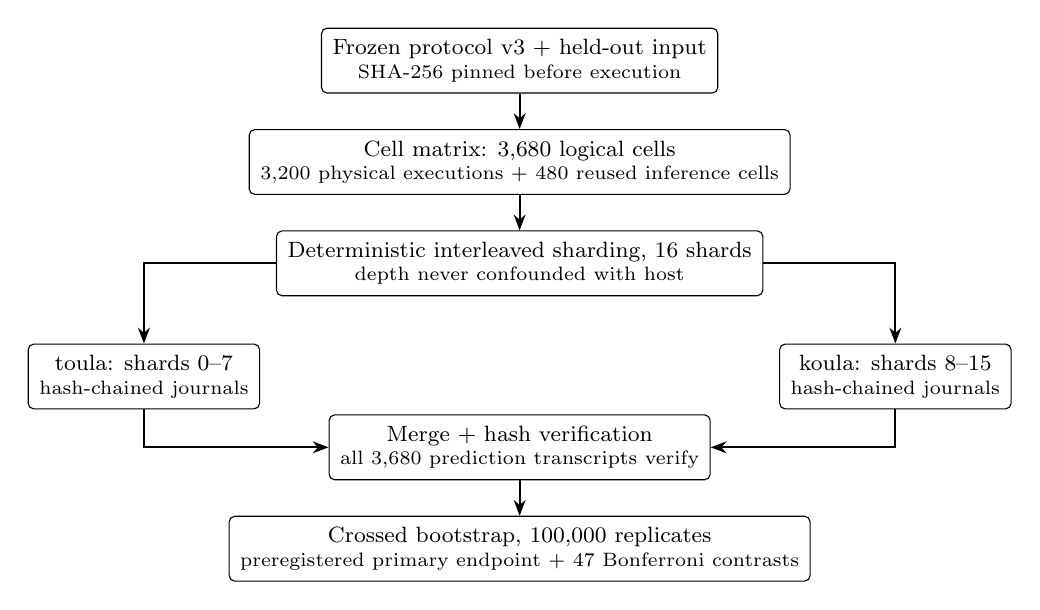
\begin{tikzpicture}[
  font=\footnotesize,
  box/.style={draw, rounded corners=2pt, align=center, inner sep=4pt},
  arr/.style={-{Stealth[length=2mm]}, thick},
  node distance=4.5mm]
\node[box] (proto) {Frozen protocol v3 + held-out input\\[-1pt]
  \scriptsize SHA-256 pinned before execution};
\node[box, below=of proto] (matrix) {Cell matrix: 3{,}680 logical cells\\[-1pt]
  \scriptsize 3{,}200 physical executions + 480 reused inference cells};
\node[box, below=of matrix] (shard) {Deterministic interleaved sharding, 16 shards\\[-1pt]
  \scriptsize depth never confounded with host};
\node[box, below left=6mm and 2mm of shard] (toula) {toula: shards 0--7\\[-1pt]
  \scriptsize hash-chained journals};
\node[box, below right=6mm and 2mm of shard] (koula) {koula: shards 8--15\\[-1pt]
  \scriptsize hash-chained journals};
\node[box, below=15mm of shard] (merge) {Merge + hash verification\\[-1pt]
  \scriptsize all 3{,}680 prediction transcripts verify};
\node[box, below=of merge] (analysis) {Crossed bootstrap, 100{,}000 replicates\\[-1pt]
  \scriptsize preregistered primary endpoint + 47 Bonferroni contrasts};
\draw[arr] (proto) -- (matrix);
\draw[arr] (matrix) -- (shard);
\draw[arr] (shard) -| (toula);
\draw[arr] (shard) -| (koula);
\draw[arr] (toula) |- (merge);
\draw[arr] (koula) |- (merge);
\draw[arr] (merge) -- (analysis);
\end{tikzpicture}
\caption{Orchestration of the 16-shard v3 validation campaign. Every stage
emits or consumes hash-pinned artefacts, so the path from frozen protocol to
published table is re-verifiable end to end. As documented in \texttt{docs/evidence-release-v3.md}, the verification of the original unmerged shards is complete, and the collision-corrected merged package (deterministic per-shard sidecar destinations, fail-closed on divergent content) hash-verifies every repository-resident reference: all 3{,}680 prediction references, the protocol/input triple, and all 17 hash-chained journals; its 860 binary-tier references were subsequently recovered and hash-verified for the pinned HF baseline release. Byte verification is distinct from regenerating predictions.}
\label{fig:v3pipeline}
\end{figure}

We froze the third validation protocol (v3) before execution, with the following primary endpoint: at depth $L{=}6$ under the public head, joint true-gradient reconstruction (\texttt{joint\_true\_k32}) must exceed the forward-only baseline (\texttt{forward\_k32}) by more than two percentage points of token accuracy, judged on the lower bound of a 95\% crossed-bootstrap confidence interval.

The campaign comprised 3{,}680 logical evaluation cells -- 3{,}200 physical executions plus 480 reused inference cells -- spanning 40 attack arms (28 undefended and 12 defended experimental conditions, distinct from the registry modules counted above), ten victim seeds, two attack seeds, depths $L \in \{3, 6\}$, and public and exact attacker knowledge, with 256 held-out documents per cell. Deterministic interleaved sharding partitioned the cell matrix across 16 shards on two GPU hosts (336.1 hours of summed, non-reused online attack wall-clock time), with depth never confounded with host. All 16 final shards completed with no missing final cells; earlier aborted shard attempts were superseded for operational reasons and are documented, with the full restart history, in the campaign's execution record.

The victim is GPT-2 (124M, revision \texttt{607a30d7}) on pinned 32-token WikiText-2 inputs with 32 calibration, 128 victim-training and 256 evaluation documents. Public knowledge grants the pretrained head; exact knowledge grants the post-training victim head. Evaluation tokens are used for scoring, not passed to the attacker. These are fixed-state post-training probes: the training condition exposes the next-token-loss gradient, and the inference condition exposes activations only. They do not measure a live training trajectory.

The frozen endpoint was met. Joint observation recovered $97.38\%$ of tokens against $94.20\%$ for the forward-only baseline at $L{=}6$ ($+3.17$ points, 95\% CI $[+2.72, +3.64]$, preregistered margin $+2$), and all 47 secondary contrasts survived Bonferroni correction. The control conditions separated information from perturbation: shuffled or random gradients collapse the joint advantage to the forward-only level ($94.2\%$), whereas the point estimates under Gaussian noise of scale $\sigma{=}0.1$ ($97.31\%$) and eight-bit quantisation ($97.33\%$) of the backward wire are close to the true-gradient result ($97.38\%$). These perturbation comparisons are descriptive: the frozen inferential family contains no equivalence test, and they measure what the attacker observes, not the utility of training with perturbed gradients.

Two prespecified defended arms were evaluated as paired descriptive comparisons. Across the evaluated secret-mixup conditions, token recovery ranged from $83.01\%$ to $90.67\%$ and exact-sequence recovery reached at most $1.48\%$; separate utility measurements, taken under a different release schedule from the reconstruction probes, showed geometric-mean perplexity increases of $31.8\%$ (depth 3) and $26.9\%$ (depth 6). Replica-median left token recovery within two-thirds of a percentage point of the undefended arms, although exact-sequence recovery moved by up to $7.7$ points in the most affected condition (public depth-3 SIPIT-128: $43.77\%$ to $36.11\%$).

\begin{table}[t]
\centering\small
\caption{The v3 primary arms by depth and knowledge condition: token
accuracy, with exact-sequence recovery as a descriptive companion. Each
entry aggregates 5{,}120 document-level evaluations over 256 distinct
held-out documents. The same campaign supplies Paper~A's confirmatory
table; both papers draw on this single canonical evidence base.}
\label{tab:v3primary}
\begin{tabular}{@{}llcccc@{}}
\toprule
 & & \multicolumn{2}{c}{\textbf{Token accuracy}} &
 \multicolumn{2}{c}{\textbf{Exact-sequence (descr.)}} \\
\cmidrule(lr){3-4} \cmidrule(lr){5-6}
\textbf{Depth} & \textbf{Knowledge} & \textbf{Forward-only} & \textbf{Joint} &
\textbf{Forward-only} & \textbf{Joint} \\
\midrule
$L{=}3$ & public & 97.39\% & 98.29\% & 43.13\% & 55.51\% \\
$L{=}3$ & exact  & 97.81\% & 98.72\% & 51.41\% & 66.13\% \\
$L{=}6$ & public & 94.20\% & 97.38\% & 13.71\% & 37.77\% \\
$L{=}6$ & exact  & 94.81\% & 98.27\% & 20.23\% & 58.55\% \\
\bottomrule
\end{tabular}
\end{table}

Every shard emitted a strict evidence-chained record (\texttt{validation.json.evidence.jsonl}); all 3{,}680 prediction transcripts hash-verify against their manifests, and the binary capture artefacts are included in the verified HF baseline, with an artefact index, checksums, and verification recipe recorded in the project repository (\texttt{docs/evidence-release-v3.md}). This campaign is the single canonical evidence source for the joint-observation reconstruction result: the companion empirical paper reports the same campaign as its confirmatory core, and the two papers are explicit that they share that evidence base rather than offering independent replications. The campaign combines a frozen protocol, a preregistered margin, multiplicity-controlled secondary analyses and an artefact chain that another evaluator can verify.

\subsection{Corrected White-Box Evaluation Across Internal Boundaries}
\label{sec:whitebox}
The earlier adaptive white-box objective applied the defence encoder directly to optimised token embeddings, omitting the client head. Its low recovery was therefore an invalid attack result, not a privacy bound. The correction optimises the full path, token embeddings $\rightarrow$ client head $\rightarrow$ true encoder $\rightarrow$ observed wire, retaining gradient flow through the client head and separately counting optimisation and vocabulary-readout work. Twenty PyTorch regression checks cover gradient traversal, compute accounting and matched final-state captures.

\paragraph{Matched rerun and fresh sweep.}
The corrected matched rerun reuses the original inputs, captures, checkpoints and budgets for 36 evaluable cells at depths three and six. Historical results remain invalid, and the 18 historical co-trained cells remain NOT\_EVALUABLE because their training-time wires lack matching encoder checkpoints. The subsequent fresh stable-defence grid covers every internal GPT-2 boundary, depths 1--11, with three seeds (11, 22, 33), PCA compression and a frozen trained bottleneck, and dimensions 64, 128 and 256: 198 cells. Eleven engineering canaries are excluded; depth twelve is not an internal boundary and no endpoint-control result is claimed. These are development-corpus measurements, not the v3 held-out confirmatory campaign.

The protocol pins GPT-2 revision \texttt{607a30d7} and the development corpus hash, with 32-token sequences, 64 victim-training steps, 32 calibration sequences, 32 attacked sequences and 128 optimisation steps. The optimisation learning rate is 0.05; the victim learning rate is $5\times10^{-5}$. The stable tier grants the public pretrained head and the true fixed defence encoder on fresh training captures. Every reported cell scores 1{,}024 token positions. Table~\ref{tab:whitebox} gives descriptive means over all three seeds and three widths; it does not pool independent corpora or support a new privacy-gate verdict.

\paragraph{Co-trained final-state tier.}
A separate 99-cell tier uses all eleven depths, three seeds and three widths. It trains a co-trained bottleneck, then captures held-out inference observations from the final victim state without optimiser updates. Each wire must replay exactly at stored precision using the saved final victim head and final encoder; the full victim checkpoint and capture identities are retained. This grants stronger model knowledge and changes observation phase relative to the stable training tier. It supplies new evidence; the 18 historical cells remain excluded.

\begin{table}[ht]
\centering\small
\caption{Corrected white-box token recovery (\%), mean across three seeds and three widths at each depth. Stable PCA and frozen-bottleneck columns use training observations and a public head; co-trained final inference grants the final victim head. Columns are separate descriptive experiments, not matched defence rankings.}
\label{tab:whitebox}
\begin{tabular}{rrrr}
\toprule
Depth & Stable PCA & Frozen bottleneck & Co-trained final inference \\
\midrule
1 & 59.16\% & 60.36\% & 61.14\% \\
2 & 66.86\% & 68.59\% & 67.68\% \\
3 & 58.32\% & 58.00\% & 60.24\% \\
4 & 56.88\% & 57.35\% & 60.22\% \\
5 & 55.90\% & 57.02\% & 56.80\% \\
6 & 50.89\% & 52.16\% & 53.09\% \\
7 & 48.94\% & 49.73\% & 48.01\% \\
8 & 41.66\% & 42.05\% & 41.10\% \\
9 & 38.82\% & 37.96\% & 38.24\% \\
10 & 31.01\% & 31.80\% & 30.31\% \\
11 & 18.85\% & 19.67\% & 23.52\% \\
\bottomrule
\end{tabular}
\end{table}

The matched original-36 means at depth three are 58.32\% (PCA) and 58.00\% (frozen bottleneck), and at depth six 50.89\% and 52.16\%, respectively. The complete fresh grid has no missing cells. Every full-grid cell records 128 head forward and backward calls, 131{,}072 head token positions in each direction and 51{,}463{,}168 vocabulary dot products in readout. Summed attack wall time is 1{,}223.24 seconds for the 198 stable cells (optimisation plus readout) and 617.16 seconds for the 99 co-trained cells. These measured times exclude victim training, capture generation, canaries and packaging; operation counts are not FLOP estimates. The source freeze and complete per-cell work records are retained in the supplement.

\subsection{Sequence-Length, Dialogue and Adaptive Follow-ups}
\label{sec:followups}
A separate frozen queue evaluates GPT-2 at split six with three seeds (11, 22, 33), eight training steps, a fixed 16-sequence calibration budget, and VMI under no defence or Gaussian noise $\sigma=15$. Four experiments cross code/WikiText reference corpora with sequence lengths 64 and 128; an independent dialogue experiment uses 32-token prefixes from a pinned 96-document DialogSum selection. Each experiment reports both training and inference conditions with its own control and shuffled-pair scores. The new inputs have zero exact normalised-text-hash overlap with the frozen validation partitions; this check does not establish semantic independence. Table~\ref{tab:followups} reports descriptive mean token recovery for all five experiments, with no transfer certificate or pooled gate declaration.

\begin{table}[ht]
\centering\small
\caption{New follow-up VMI recovery (\%), three-seed means. Gaussian noise is $\sigma=15$. Training and inference have distinct observation contracts; these raw rates must be read with the per-corpus controls retained in the release.}
\label{tab:followups}
\begin{tabular}{lr rrrr}
\toprule
 & & \multicolumn{2}{c}{Training} & \multicolumn{2}{c}{Inference} \\
Corpus & Tokens & None & Gaussian & None & Gaussian \\
\midrule
Code & 64 & 78.32\% & 21.55\% & 79.70\% & 26.27\% \\
Code & 128 & 87.37\% & 23.11\% & 86.71\% & 32.92\% \\
WikiText reference & 64 & 81.77\% & 9.96\% & 82.50\% & 20.82\% \\
WikiText reference & 128 & 88.96\% & 14.55\% & 90.22\% & 26.17\% \\
Dialogue & 32 & 76.56\% & 36.72\% & 76.99\% & 55.05\% \\
\bottomrule
\end{tabular}
\end{table}

The paired adaptive-whitening comparison does not uniformly strengthen the attack: Gaussian-defended inference recovery changes from 21.65\% to 13.09\%, whereas training-mode recovery changes from 11.46\% to 13.67\%. Undefended values are unchanged in these runs. These are descriptive paired observations, not an equivalence test or a claim that adaptation is ineffective in general. The released report retains all per-seed results and its intervals, which condition on fixed documents.

The synthetic order/chaff battery also completed for three paired reference-bundle seeds. Its matching arm explicitly scores permutation order separately from token identity, and its sensitivity arm includes a chaff-retaining counter-test. These bundles are framework-generated references, not the external v13 defence or a replication of published VMA. The six matching reports' worst order excesses range from 0.52 to 5.21 percentage points across reference settings and seeds. The individual arms and chaff curves are retained without promotion into a real-deployment privacy guarantee. The 500-step trajectory extension completed execution but is excluded from this release; it still requires evidence collection, independent verification and analysis.

\subsection{Matched BiSR implementation conformance}
\label{sec:bisr-conformance}
We validated the single-seam BiSR adaptation against attack methods extracted from pinned upstream SplitLLM commit \texttt{c376590}, using identical saved victim and inverter checkpoints, observations and algorithm budgets. This is the prespecified C-A implementation-conformance route, not a reproduction of the published dual-cut setting. Candidate and reference predictions ran in separate processes without scorer-only ground truth. All twelve trained depth/grant/seed mechanical gates passed before full prediction; these compare logits, losses, gradients and an optimiser update on the fixed first and last validation observations.

The frozen inputs comprise 256 fresh 32-token validation documents and 112 separate auxiliary articles, yielding 15{,}604 non-overlapping auxiliary windows. Both sets are drawn from the pinned WikiText-103 training partition, with validation held out internally; they are not the dataset's official test partition. The selection excludes the recorded historical inputs and the WikiText-2 partitions. Six GRU inverters were trained for twenty epochs. The matched design crosses depths 3 and 6, public and exact head grants, and three prespecified seeds (31415, 27182, 16180). Both engines completed all 24 prediction cells, or 6{,}144 document--engine runs, retaining SIP, b, f and bf predictions in every run. The implementation comparison shares checkpoints and inputs; it is not an independent end-to-end retraining replication.

The separate scorer verified completeness and prediction journals before evaluating positional token accuracy and ROUGE-L F1 for each of the four arms. Within each of the four depth/grant strata, all eight endpoints met the prospective equivalence rule: the 90\% Student-$t$ interval across three paired seed differences must lie strictly within $(-0.01,0.01)$. An independent audit found identical predicted token sequences for every arm in all 3{,}072 paired document runs. Every observed seed-level difference was zero, giving mean difference 0 and interval $[0,0]$ for all 32 endpoint/stratum comparisons. These degenerate intervals describe observed implementation agreement conditional on these fixed documents; they do not establish zero uncertainty on new data, architectures or split boundaries. METEOR and token-set F1 are retained as descriptive metrics, not additional equivalence endpoints.

This result closes the declared single-seam conformance requirement. It does not establish superiority over BiSR, equal compute, a matched-v4 campaign result, or reproduction of the original SensiReplaced data and published dual-cut configuration. The frozen v4 B1 gate requires that published setting and therefore remains blocked; the C-A pass alone does not admit it. Per-stage wall time, peak allocated memory and transformer-layer forward/reverse token-position counts are retained separately from offline training; these counts are not FLOP estimates. Frozen predictions, checkpoints, inputs, source and environment records, mechanical traces, and the final comparison are linked in the evidence-availability paragraph below.

\section{Historical Evidence Exclusions}
\label{sec:campaign}
\label{sec:repro}
The previous draft reported numerical findings from an August deployment campaign and an external adopting defence project's v2--v13 evaluations, including latent-era PASS verdicts, compromise curves, matching results, integrity checks and a PR-101 reproduction. Their required source journals, manifests and release mapping remain unavailable in the inspected records. Those tables, abstract claims and taxonomy highlights are therefore withdrawn from this revision's active evidence; attribution to an external project does not resolve the missing provenance.

These external defence records are distinct from Paper~A's retired P0--P5 programme. Recovery of P0--P5 files does not fill the v5--v13 or August deployment gaps, and successful new synthetic reference-bundle tests do not reproduce the adopting project's boundary. We also withdraw the reviewer response's unsupported claim that those exploratory results were transformed into the v3 confirmatory protocol. The v3 source freeze and declared endpoint stand on their own provenance record.

The original BiSR published-setting reproduction remains unestablished because the original SensiReplaced version and the published dual-cut configuration are outside the completed validation. The aligned single-seam implementation, metric gate and prospective equivalence criterion are now validated within the narrower scope of \S\ref{sec:bisr-conformance}. This result does not retroactively validate the historical substitute runs.

\section{Related Work}
\label{sec:related}

\paragraph{Split-learning privacy attacks.}
Gradient inversion began with DLG \cite{dlg} and its analytic label recovery
(iDLG) \cite{idlg}, extended with gradient-prior regularisation
(GradInversion) \cite{gradinversion} and
transformer-specific direction decodes (TAG \cite{tag}; LAMP \cite{lamp}); the framework's
\attack{gradient-inversion} module implements all three arms plus a
DLG++ solver. Norm-based property scoring on gradients
\cite{normscore} underpins \attack{label-scoring}, and the ExPLoit
batch-label-inference line \cite{bli} underpins \attack{batch-label-recon}.
Output-side inversion follows the SipIt injectivity line
\cite{sipit}, extending the earlier LLM-inversion result
\cite{morris2024llminv} (\attack{output-inversion}); seam inversion provides a clean-room implementation of the VFLAIR-LLM
VMI/WhiteBoxInversion family \cite{vflair}
(\attack{seam-inversion}), with \attack{vec2text-inversion} upgrading the
decode from nearest-neighbour to a learned generator with iterative
correction (vec2text line \cite{vec2text}). The framework includes a single-seam adaptation of BiSR (\attack{bisr-baseline}), with matched implementation conformance established in \S\ref{sec:bisr-conformance}. Reproduction of the published setting and a matched confirmatory comparison against \cite{bisr2024} remain outstanding. The pre-LLM
literature established model inversion, model stealing, and label
inference against two-party splits (FSHA \cite{pasquini2021unleashing};
UnSplit \cite{erdogan2022unsplit}), and recent internal-state inversion
shows that depth alone does not ensure privacy \cite{dong2025depth}, motivating evaluation across internal boundaries.

\paragraph{Matching and permutation attacks.}
\attack{latent-matching} implements VMA-style centroid vocabulary matching
(Hidden No More, ICML'25 \cite{hiddennomore}) and the position-free
signature family \cite{sigmatch} that reversed PermLLM- \cite{permllm_zhang},
STIP- \cite{permlmm}, and Centaur-style
permutation defences. The ICML'25 paper and arXiv:2505.18332 are the
published and preprint versions of the same work, as its arXiv record
documents; we cite both because the two arms quote different versions.
The framework exposes both arms, but this revision makes no verified claim about the external adopting project's boundary.

\paragraph{Membership inference.}
\attack{lira-membership} follows LiRA \cite{lira} with an RMIA
offline-quantile scoring arm \cite{rmia}, with null-world controls; no matched superiority result is claimed here. Property inference beyond the task label has longstanding
precedent \cite{melis2019}; \attack{label-scoring} is the framework's
property-inference arm on gradients.

\paragraph{Malicious servers.}
\attack{active-cloud} and \attack{malicious-server} transplant the
federated malicious-server line \cite{boenisch,fowl} to split
training: crafted model/body computations that steer the client into
leaking under explicit intervention and observation grants; the historical fleet effect size is excluded.

\paragraph{Side channels.}
\attack{gpu-memory} follows LeftoverLocals \cite{leftoverlocals} for allocator
residue and adds a unified-memory bandwidth-contention channel in the
GPU.zip line \cite{gpuzip};
\attack{kv-timing} implements the KV/prefix-cache TTFT channel
\cite{kvleak} plus a speculative-decoding acceptance-pattern
arm; \attack{wire-shape} performs traffic-shape analysis following NetEcho.

\paragraph{Reasoning theft.}
\attack{reasoning-replay} and \attack{trace-inversion} implement the
stolen-thoughts and trace-inversion \cite{traceinv} families against
opaque provider chain-of-thought blobs and hidden traces, scored as
capability-excess over answer-only controls under the same frozen gate.

\paragraph{Application-profile and agentic checks.}
The application-profile family follows the indirect prompt-injection line
\cite{greshake2023not}, with retrieval and grounding coverage scored in
the style of agentic benchmarks and scanners \cite{trivedi2024appworld,garak2024};
the agentic family is indexed to the OWASP agentic-security catalogue
\cite{owasp2026asi}. Both report defended-vs-vulnerable toy-world
contrasts, not campaign numbers (\S\ref{sec:framework}).

\paragraph{Methodology.}
The frozen-gate approach follows evaluation principles used in membership
inference and cryptography: specify and version the attacker and scoring
rule, then keep them fixed while evaluating defences. Capture, label and key-budget sweeps can extend point measurements into breakdown curves, provided their source evidence and observation contracts are retained.

\section{Conclusion}
\label{sec:conclusion}

LLM-Attacker supplies a common execution and evidence interface for 64 registered modules, with explicit observation grants and versioned scoring. Its strongest confirmatory evidence here is the frozen v3 reconstruction contrast. Separate domain, horizon and corrected white-box experiments demonstrate additional uses while retaining their descriptive scope. The matched BiSR validation establishes implementation conformance for the declared single-seam configuration on fixed inputs. The corrected objective and excluded historical observations illustrate why an intact evidence chain cannot compensate for an invalid attack or missing execution provenance. The framework's coverage is broader than its empirical validation, and unsupported historical campaign claims are not part of this revision's conclusions.

\paragraph{Evidence availability.}
The baseline is archived in the public dataset \href{https://huggingface.co/datasets/Setloop/llm-attacker-paper-b/tree/9833a3df9c660a6b214336d029095c46224c6987}{Setloop/llm-attacker-paper-b at revision \texttt{9833a3df}}; its audit supplement is verified at \texttt{5b2e47c6}. The baseline manuscript and claim index predate this correction and are superseded by the revision index. The baseline contains v3 predictions, journals and binary captures; domain, horizon and clustered analyses; live-planner records; positive controls; code, protocols and inputs. Their paths and checksums are indexed in \nolinkurl{docs/evidence-release-hf.md} and the archive's manifests.

The corrected original-36 white-box package is remotely verified at \href{https://huggingface.co/datasets/Setloop/llm-attacker-paper-b/tree/ba37427807a29f217e6fefb565c5e468e9bdac81/whitebox35-20260917/original36}{revision \texttt{ba374278}, original36 tier}. The full all-boundary white-box package is verified at \href{https://huggingface.co/datasets/Setloop/llm-attacker-paper-b/tree/08ed4bd07ecde7613eff62826f6cce6638415d7b/whitebox35-20260917/full}{revision \texttt{08ed4bd0}, full tier} (31 files). The Phase~2 raw supplement is verified at \href{https://huggingface.co/datasets/Setloop/llm-attacker-paper-b/tree/7aac5e7b1e9db9978ef1ef1366eb9bc5a4637ed4/revision-20260917/phase2-raw}{revision \texttt{7aac5e7b}, Phase~2 raw tier} (four files, 7.15\,GB). These verified releases retain their stated exclusions; publication does not qualify incomplete or invalid experiments.

The BiSR conformance package is archived under \href{https://huggingface.co/datasets/Setloop/llm-attacker-paper-b/tree/be59bdca280258ac82ce358cae5f1e0c529869c2/fidelity-20260919/evidence}{\texttt{fidelity-20260919} at its immutable release revision}. Its manifest binds the frozen inputs, predictions and journals, trained checkpoints, source commits, environment, measured work and final analysis; the package README gives verification, rescoring and regeneration instructions. Its scope is the completed C-A validation, with original-setting exclusions retained.

\paragraph{Reproduction.}
Install the archived source and research dependencies in an isolated environment. The CLI provides \texttt{--self-test}, \texttt{--list-attacks}, \texttt{--scorecard}, \texttt{--coverage} and \texttt{--profiles}; toy-tier tests do not require PyTorch. The source's \texttt{verify\_evidence} checks the retained chains and artefact digests. Verification, prediction rescoring and regeneration are different operations, as specified in \nolinkurl{docs/evidence-release-v3.md}. The corrected white-box archive includes its protocol, source, input hashes, captures, checkpoints and measured work, with regeneration commands in its README. Publication and interpretation gaps are stated in \nolinkurl{docs/paper-b-closure-2026-09-17.md}; no claim is made that every module is a faithful reproduction of its motivating paper.

\input{main.bbl}

\end{document}
